\documentclass[dvipdfmx,autodetect-engine]{jsarticle}% 適切なドライバ指定が必要
\usepackage[svgnames]{xcolor}% tikzより前に読み込む必要あり
\usepackage{tikz}

\begin{document}

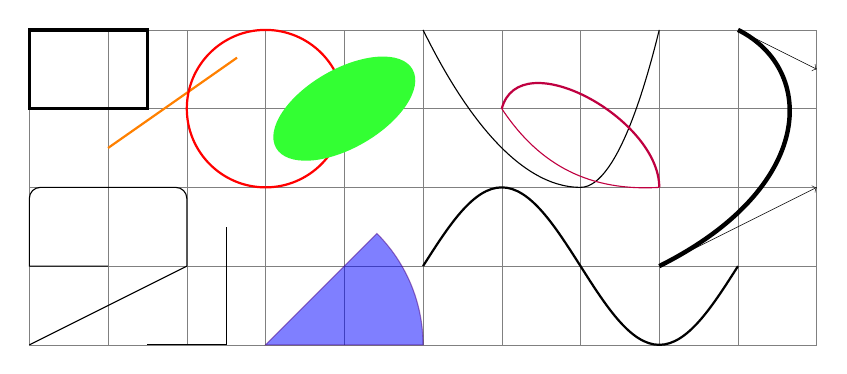
\begin{tikzpicture}
\draw [help lines] (0,0) grid (10,4);%(0,0)から(10,4)までの"細線の方眼"

%%直線の例
\draw (0,0) -- (2,1)  [rounded corners]--(2,2) -- (0,2) [sharp corners] --  (0,1)-- (1,1);
   %点(0,0), (2,1), (2,2), (0,2), (0,1), (1,1)を結ぶ"線分"で,(2,2)と(0,2)では"滑らか"
\draw [orange, thick] (1,2.5) -- ++(35:2cm);
   %(1,2.5)を始点として35°の方向に2cmの"オレンジ色の太い線分"
\draw [very thick] (0,3) rectangle (1.5,4);
   %(0,3)を左下,(1.5,4)を右上とする"極太の長方形"
\draw (1.5,0) -| (2.5,1.5);
   %(2,0)と(3,1.5)をまっすぐ結ばずに"横線と縦線のみで結ぶ"

%%円,楕円,扇形
\draw [red, thick] (3,3) circle (1);
   %(3,3)を中心とする半径1の"赤い太線の円"(古い書式で,現在は非推奨)
\fill [green!80] (4,3) circle [x radius=1cm, y radius=5mm, rotate=30];
   %中心(4,3),横1cm,縦5mmの"楕円を30°傾け緑80%で塗った図形"(推奨されている新しい円の書式)
\filldraw [fill=blue, opacity=.5, draw=Indigo] (5,0)  arc (0:45:2) --(3,0)--cycle;
   %(5,0)を出発点に半径2の弧を0°から45°まで描き,(3,0)を経由して出発点まで線分で戻って囲んだ"透明度50%の青で塗った扇形"
%%放物線,サインカーブ,曲線,ベジェ曲線
\draw (5,4) parabola bend (7,2) (8,4);
   %(5,4)を始点とし(7,2)を頂点とする放物線と(7,2)を頂点とし(8,4)を終点とする"放物線"
\draw [thick] (5,1) sin (6,2) cos (7,1) sin (8,0) cos (9,1);
   %(5,1)から始まり,(6,2),(8,0)を頂点として(9,1)で終わる"太線のサインカーブ"
\draw [purple, thick] (6,3) to [out=75, in=90] (8,2);
   %(6,3)から75°の角度で出発し,90°の角度で終点(8,3)に至る"紫の太い曲線"
\draw [purple, thin, bend right = 30] (6,3) to (8,2);
   %2点(6,3)と(8,2)を結ぶ"右に膨らんだ紫の細い曲線"(30°の角度で始点を出発し,150°の角度で終点に至る)
\draw [ultra thick] (8,1) .. controls (10,2) and (10,3.5) ..(9,4);
   %始点(8,1),終点(9,4)で方向点がそれぞれ(10,2)と(10,3)である"超極太の3次ベジェ曲線"
\draw [->, very thin]    (8,1) -- (10,2); \draw[<-, very thin] (10,3.5) -- (9,4);
   %上のベジェ曲線の"→つき方向線を示した細線"
\end{tikzpicture}

%%関数による描画(マニュアルp.329の例)
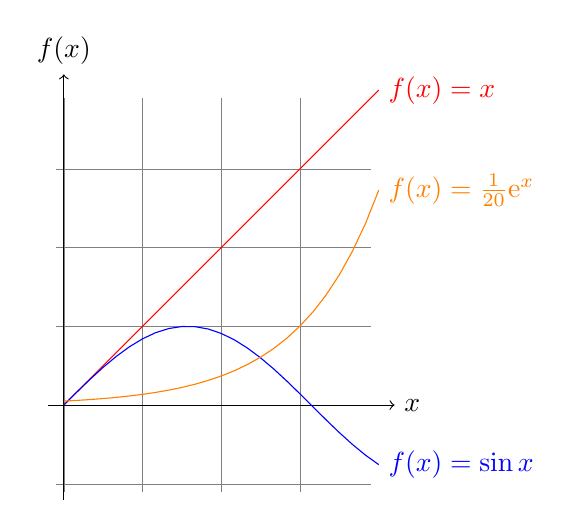
\begin{tikzpicture}[domain=0:4]%グラフの描画領域は0≦x≦4
\draw[very thin,color=gray] (-0.1,-1.1) grid (3.9,3.9);
\draw[->] (-0.2,0) -- (4.2,0) node[right] {$x$};%横軸(x軸)
\draw[->] (0,-1.2) -- (0,4.2) node[above] {$f(x)$};%縦軸
\draw[color=red] plot (\x,\x) node[right] {$f(x) =x$};
   %一次関数 y=x の赤線
% \x r means to convert '\x' from degrees to _r_adians:
\draw[color=blue] plot (\x,{sin(\x r)}) node[right] {$f(x) = \sin x$};
   %三角関数 y=sin x の青線(度数表記→ラジアンに変換)
\draw[color=orange] plot (\x,{0.05*exp(\x)}) node[right] {$f(x) = \frac{1}{20} \mathrm e^x$};
   %指数関数 y=0.05e^x のオレンジの線
\end{tikzpicture}



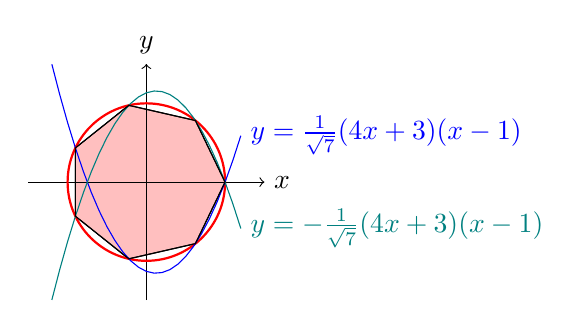
\begin{tikzpicture}[domain=-1.2:1.2]
\filldraw[fill=pink,domain=0:360,samples=8] plot({cos(\x)}, {sin(\x)});
%\draw[very thin,color=gray] (-1.2,-1.2) grid (1.2,1.2);
\draw[->] (-1.5,0) -- (1.5,0) node[right] {$x$};
\draw[->] (0,-1.5) -- (0,1.5) node[above] {$y$};
\draw [red, thick] (0,0) circle (1);
%\draw [red, thick] (0,0) circle [x radius=1cm, y radius=1cm];
\draw[color=blue] plot (\x,{(4*\x*\x-\x-3)/sqrt(7)}) node[right] {$y = \frac{1}{\sqrt{7}}(4x+3)(x-1)$};
\draw[color=teal] plot (\x,{-(4*\x*\x-\x-3)/sqrt(7)}) node[right] {$y = -\frac{1}{\sqrt{7}}(4x+3)(x-1)$};
\draw[color=black,domain=0:360,samples=8] plot({cos(\x)}, {sin(\x)});
\end{tikzpicture}


\end{document}
